\documentclass[10pt,a4paper, margin=1in]{article}
\usepackage{fullpage}
\usepackage{amsfonts, amsmath, pifont}
\usepackage{amsthm}
\usepackage{graphicx}
\usepackage{float}
\usepackage{geometry}
\usepackage{tkz-euclide}
\usepackage{tikz}
\usepackage{pgfplots}
\pgfplotsset{compat=1.13}
 \geometry{
 a4paper,
 total={210mm,297mm},
 left=10mm,
 right=10mm,
 top=10mm,
 bottom=10mm,
 }
 % Write both of your names here. Fill exxxxxxx with your ceng mail address.
 \author{
  Öztürk, Kürşat\\
  \texttt{e2171874@ceng.metu.edu.tr}
  \and
  Burhan, Beste\\
  \texttt{e2171395@ceng.metu.edu.tr}
}
\title{CENG 384 - Signals and Systems for Computer Engineers \\
Spring 2018-2019 \\
Written Assignment 1}
\begin{document}
\maketitle



\noindent\rule{19cm}{1.2pt}

\begin{enumerate}

\item 
    \begin{enumerate}
    % Write your solutions in the following items.
    \item %write the solution of q1a
    \  \\
    $i)$\\
    $z=x+jy$\\
    $\bar{z}=x-jy$\\
    $3z+4=2j-\bar{z}$\\
    $3z+\bar{z}=2j-4$\\
    $4x+2yj=2j-4$\\
    $y=1$\\
    $x=-1$\\
    $z=-1+j$\\
    $|z|^2=2$\\
    \ \\
    $ii)$\\
    \begin{figure}[h!]
    	\centering
    	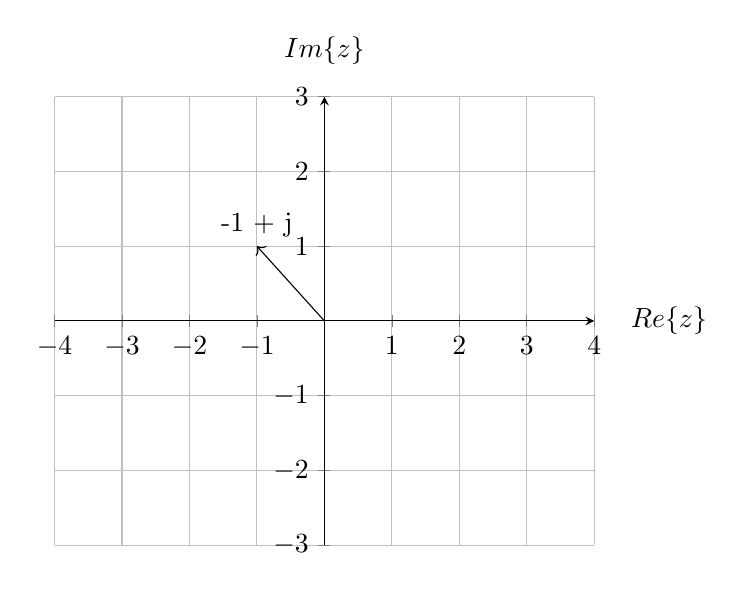
\begin{tikzpicture}[scale=1.0]
    	\begin{axis}[
    	axis lines=middle,
    	xlabel={$Re\{z\}$},
    	ylabel={${Im\{z\}}$},
    	xtick={-4, -3, -2, -1, ..., 4},
    	ytick={-3, -2, -1, ..., 3},
    	ymin=-3, ymax=3,
    	xmin=-4, xmax=4,
    	every axis x label/.style={at={(ticklabel* cs:1.05)}, anchor=west,},
    	every axis y label/.style={at={(ticklabel* cs:1.05)}, anchor=south,},
    	grid,
    	]
    	%\path[draw,line width=1.5pt] (-1,1) -- (0,0);
    	\draw[->,black] (0,0) -- (-1, 1) node [sloped, above] {-1 + j};
    	
    	\end{axis}
    	\end{tikzpicture}
    	\caption{$Re\{z\}$ vs. $Im\{z\}$.}
    	\label{fig:q2}
    \end{figure}


    
    \item %write the solution of q1b
    \ \\
    	$z = r e^{j\theta}$\\
    	$z^3 = 64j$\\
    	$z^3 = r^3 e^{3j\theta}$\\
    	$64j = r^3 e^{3j\theta}$\\
    	$64j = r^3 (cos(3\theta) + jsin(3\theta))$\\
    	$64j = 64 (cos(\pi/2+2\pi k) + jsin(\pi/2+2\pi k))$\\
    	$z = \sqrt[3]{64}[cos(\frac{\pi/2+2\pi k}{3})+jsin(\frac{\pi/2+2\pi k}{3})]$\\
    	$z_1 = 4[cos(\pi / 6) + jsin(\pi / 6)] = 2\sqrt{3} + 2j $\\
    	$z_1 = 4[cos(5\pi / 6) + jsin(5\pi / 6)] = -2\sqrt{3} + 2j $\\
    	$z_1 = 4[cos(3\pi/2) + jsin(3\pi/2)]= -4j $ \\
   	\\
    \item %write the solution of q1c
    \ \\
   		$z= \frac{(1-j)(1+\sqrt{3}j)}{1+j}$ \\
   		$z = \frac{\sqrt{2}e^{j7\pi/4} * 2e^{j\pi / 3}}{\sqrt{2} * e^{j\pi/4}} $ \\
   		$z = 2e^{(7\pi/4 + \pi/3 - \pi/4)j}$ \\
   		$z = 2e^{j11\pi/6 }$ \\
   		magnitude = 2 \\
   		angle = $11\pi/ 6$
    \item %write the solution of q1d
	\ \\
	$z=-je^{j\pi/2}$\\
	$z=e^{j3\pi/2}e^{j\pi/2}$\\
	$z=e^{j2\pi}$\\
	$z=cos(2\pi) + jsin(2\pi)$\\
	    



\end{enumerate}


\item %write the solution of q2
\ \\
\begin{figure}[h!]
	\centering
	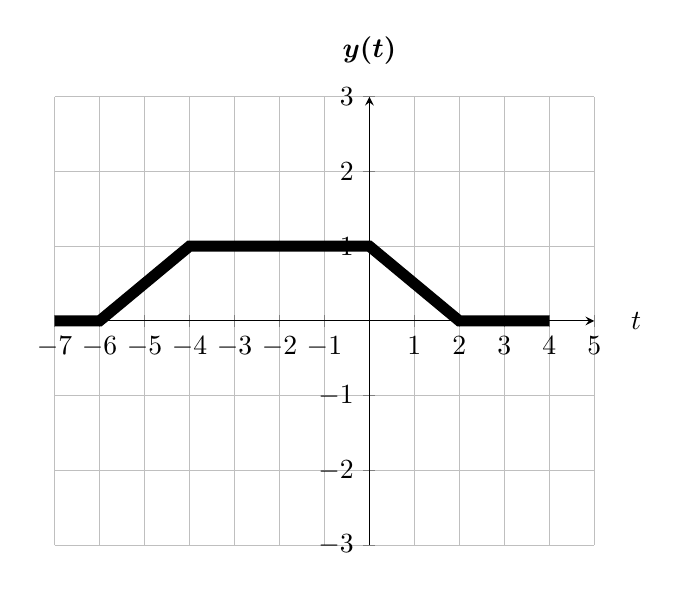
\begin{tikzpicture}[scale=1.0]
	\begin{axis}[
	axis lines=middle,
	xlabel={$t$},
	ylabel={$\boldsymbol{y(t)}$},
	xtick={-7, -6, -5, -4, ..., 5},
	ytick={-3, -2, -1, ..., 3},
	ymin=-3, ymax=3,
	xmin=-7, xmax=5,
	every axis x label/.style={at={(ticklabel* cs:1.05)}, anchor=west,},
	every axis y label/.style={at={(ticklabel* cs:1.05)}, anchor=south,},
	grid,
	]
	\path[draw,line width=4pt] (-7,0) -- (-6, 0) -- (-4, 1) -- (0, 1) -- (2,0) -- (4,0);
	\end{axis}
	\end{tikzpicture}
	\caption{$t$ vs. $y(t)=x(t/2 + 1))$.}
	\label{fig:q2}
\end{figure}

\item      
    \begin{enumerate}
    \item %write the solution of q3a
    \ \\
    \begin{figure}[h!]
    \centering
    \begin{tikzpicture}[scale=1.1] 
    \begin{axis}[
    axis lines=middle,
    xlabel={$n$},
    ylabel={$\boldsymbol{x[-n]+x[2n+1]}$},
    xtick={ -8, -7, ..., 8},
    ytick={-5,-4.5,-4,-3.5 ,-3, -2.5, -2, -1.5, -1, -0.5, ..., 4},
    ymin=-5, ymax=4,
    xmin=-8, xmax=4,
    every axis x label/.style={at={(ticklabel* cs:1.05)}, anchor=west,},
    every axis y label/.style={at={(ticklabel* cs:1.05)}, anchor=south,},
    grid,
    ]
    \addplot [ycomb, black, thick, mark=*] table [x={n}, y={xn}] {q3a.dat};
    \end{axis}
    \end{tikzpicture}
    \caption{$x[-n]+x[2n+1]$.}
    \label{fig:q3}
\end{figure}
    \item %write the solution of q3b
    \ \\
    $x[n]+x[2n+1] = 3\delta(n+7)-4\delta(n+4)+2\delta(n+2)-\delta(n+1)-\delta(n)+3\delta(n-3)$
    \end{enumerate}

\item 
\ \\
    \begin{enumerate}
    \item %write the solution of q4a
    \ \\
    	$x[n] = 3x_1[n] + 5x_2[n]$ \\
    	where\\
    	 $x_1[n] = cos[13\pi / 10 n]$ and $x_2[n] = cos[7\pi /3 - 2\pi /3]$ \\
    	$w_1 = 13\pi/10$ \\
    	$T_1 = 2\pi / (13\pi/10)$ \\
    	$T_1 = 20/13$ \\
    	$w_2 = 7\pi/3$ \\
    	$T_2 = 2\pi/ (7\pi/3)$ \\
    	$T_2 = 6/7$ \\
    	$T_1/T_2 = \frac{20/13}{6/7} = 70/39 $\\
    	$T_0 = 39 * 20/13 = 60 $\\
    	So it is periodic and its period is 60.
    \item %write the solution of q4b
    $w_1=3$ \\
    $T_1 = 2\pi/ 3$\\
    Since there is not an integer m such that $ 2\pi/ 3 * m$ is integer, y[n] is not periodic. \\ 
    \item %write the solution of q4c
    $w_1=3\pi$ \\
    $T_1 = 2\pi/ 3\pi$\\
    $T_1 = 2/3 $ \\
    Since there is an integer m such that 2/3 * m is integer, y[n] is periodic and its period is 2. \\
    \item %write the solution of q4d
    $x(t) = e^{(3\pi/2)j}e^{5tj}$ \\
    $x(t) = e^{(5t+3\pi/2)j}$\\
    $w_1 = 5$ \\
    $T_1 = 2\pi/5 $ \\
    $x(t)$ is periodic and its period is $2\pi/5$ \\
    \end{enumerate}

\item %write the solution of q5
\ \\
$Ev\{x[n]\} = 1/2\{x[n] + x[-n]\} $\\

\begin{tikzpicture}[scale=1.1] 
\begin{axis}[
axis lines=middle,
xlabel={$n$},
ylabel={$\boldsymbol{x[n]}$},
xtick={ -8, -7, ..., 8},
ytick={-3, -2.5, -2, -1.5, -1, -0.5, ..., 3},
ymin=-3, ymax=3,
xmin=-8, xmax=8,
every axis x label/.style={at={(ticklabel* cs:1.05)}, anchor=west,},
every axis y label/.style={at={(ticklabel* cs:1.05)}, anchor=south,},
grid,
]
\addplot [ycomb, black, thick, mark=*] table [x={n}, y={xn}] {q5ev.dat};
\end{axis}
\end{tikzpicture}


$Od\{x[n]\} = 1/2\{x[n] - x[-n]\} $\\

\begin{tikzpicture}[scale=1.1] 
\begin{axis}[
axis lines=middle,
xlabel={$n$},
ylabel={$\boldsymbol{x[n]}$},
xtick={ -8, -7, ..., 8},
ytick={-3, -2.5, -2, -1.5, -1, -0.5, ..., 3},
ymin=-3, ymax=3,
xmin=-8, xmax=8,
every axis x label/.style={at={(ticklabel* cs:1.05)}, anchor=west,},
every axis y label/.style={at={(ticklabel* cs:1.05)}, anchor=south,},
grid,
]
\addplot [ycomb, black, thick, mark=*] table [x={n}, y={xn}] {q5od.dat};
\end{axis}
\end{tikzpicture}

\item 
    \begin{enumerate}
    \item %write the solution of q6a
    \ \\
    Memoriless:\\
    
    y(t) has memory because y(t) depends on previous  and next values of x(t). For example: y(1) = x(-1),
     y(4) = x(5)\\
     
     Stability: \\
     
     if $|x(t)|\textless M$, $|x(2t-3)|\textless M$ and $|y(t)|\textless M$, Then
      $y(t) = x(2t-3)$ is stable.\\
     
     Causality:\\
     
     The value of y(.) at time=4 depends on x(.) at a future time(t=5). Hence it is not causal.\\
     
     Linearity:\\
     
     $y(t) = x(2t-3) = T[x(t)]$\\
     $T[ax_1(t) + bx_2(t)] = ax_1(2t-3) + bx_2(2t-3) = aT[x_1(t)] + bT[x_2(t)]$\\
     So, y(t) is linear\\
     
     Invertibility:\\
     
     y(t) is invertible. x(t) = y($\frac{t+3}{2}$)\\
     
     Time-invariance:\\
     
     $y(t) = x(2t-3) = T[x(t)]$\\
     $T[x(t-T_0)] = x(2t-2T_0 - 3) \ne x(2t- T_0 -3) = y(t- T_0)$\\
     So y(t) is not time-invariant. \\
     
     
    \item %write the solution of q6b
    \ \\
    Memoryless:\\
    
    y(t) is memoryless because y(t) depends only on x(t), not on previous or next values.\\
    
    Stability: \\
    
   It is unstable. When t goes to $\infty$, y(t) also goes to $\infty$. \\
  
    
    Causality:\\
    
    	y(t) only depends on present values of x(t). So it is causal.\\
    	
    Linearity:\\
    
    $y(t) = tx(t) = T[x(t)]$\\
    $T[ax_1(t) + bx_2(t)] =t[ax_1(t) + bx_2(t)] = aT[x_1(t)] + bT[x_2(t)]$\\
    So, y(t) is linear\\
    
    Invertibility:\\
    
    y(t) is invertible. x(t) = $\frac{1}{t}$y(t)\\
    
    Time-invariance:\\
    
    $y(t) = tx(t) = T[x(t)]$\\
    $T[x(t-T_0)] = tx(t-T_0) \ne (t-T_0)x(t- T_0) = y(t- T_0)$\\
    So y(t) is not time-invariant. \\
    
    
    
    
    
    \item %write the solution of q6c
    
    \ \\
    Memoriless:\\
    
    y[n] has memory because y[n] depends on previous  and next values of x[n]. For example:  y[4] = x[5]\\
    
    Stability: \\
    
    if $|x[n]|\textless M$, $|x[2n-3]|\textless M$ and $|y[n]|\textless M$, Therefore
    $y[n] = x[2n-3]$ is stable.\\
    
    Causality:\\
    
    The value of y[.] at time=4 depends on x[.] at a future time(t=5). Hence it is not causal.\\
    
    Linearity:\\
    
    $y[n] = x[2n-3] = T[x[n]]$\\
    $T[ax_1[n] + bx_2[n] = ax_1[2n-3] + bx_2[2n-3] = aT[x_1[n]] + bT[x_2[n]]$\\
    So, y[n] is linear\\
    
    Invertibility:\\
    
    y[n] is not invertible. $x[n] = \delta[n] + \delta[n-1]$ and $ x_2 = \delta[n]$ will give $y[n] = \delta[n]$\\
    
    Time-invariance:\\
    
    $y[n] = x[2n+3] = T[x[n]]$\\
    $T[x[n-N_0]] = x[2n-2N_0 - 3] \ne x[2n-N_0 - 3] = y[n - N_0]$\\
    So y(t) is not time-invariant. \\
    
    
    \item %write the solution of q6d
    
    \ \\
    Memoriless:\\
    
    y[n] has memory because y[n] depends on previous values of x[n] and not present values.\\
    
    Stability: \\
    
	y[n] is unstable. , if $x[n] \le M$ and $y[n] \le M \sum_{k=1}^{\infty} 1$. It is unbounded. So y[n] is not stable.\\
    
    Causality:\\
    
    y[n] is always depends  on previous values of x[n]. It is causal. \\
    
    Linearity:\\
    
    $|y[n] = \sum_{k=1}^{\infty}x[n-k] = T[x[n]]|$\\
    $T[ax_1[n] + bx_2[n]] = a\sum_{k=1}^{\infty}x_1[n-k] + b\sum_{k=1}^{\infty}x_2[n-k] = aT[x_1[n]] + bT[x_2[n]]$\\
    So, y[n] is linear.\\
    
    Invertibility:\\
    
    y[n] is invertible. x[n] = y[n+2] - y[n+1] \\
    
    Time-invariance:\\
    
    $y[n] = \sum_{k=1}^{\infty}x[n-k] = T[x[n]]$\\
    $T[x[n-N_0]] =\sum_{k=1}^{\infty}x[n- N_0 -k] = \sum_{k=1}^{\infty}x[n - N_0 -k] = y[n - N_0]$\\
    So y[n] is time-invariant. \\
    
    
    \end{enumerate}

\end{enumerate}
\end{document}

